\section{最终效果与适用边界}
\label{sec:results}

\subsection{选定方案在预留记录上的表现}
选择阶段结束后，最终方案与参考设置一同固定，再处理600条预先保留的记录，共62,284个原始点。它们不用于修改参数、方向条件或记忆。比较仍采用原来的覆盖、共同几何、断点与P预算条件，不因最终结果改变标准。

\begin{table}[htbp]\centering\small
\caption{600条最终确认记录的处理结果}\label{tab:confirm}
\begin{tabularx}{\linewidth}{@{}Yrr@{}}\toprule
读数 & 参考设置 & 最终过滤调整\\\midrule
短段过滤点 & 26,416 & 64\\
方向删除点 & 1,845 & 2,148\\
DP精简点 & 23,032 & 47,958\\
显式保留点 & 10,991 & 12,114\\
共同覆盖点 & 35,868 & 62,220\\
无输出记录 & 255 & 0\\\bottomrule
\end{tabularx}
\end{table}

全部600条通过规定保护，其中349条共同覆盖严格增加、251条覆盖不变。新增覆盖26,352点，显式存储只增加1,123点，表明多数重新进入处理的观测仍由简化后的线段表达。图\ref{fig:confirm-hist}进一步展示增量分布，避免仅用一个总数掩盖记录之间的差异。

\begin{figure}[H]\centering
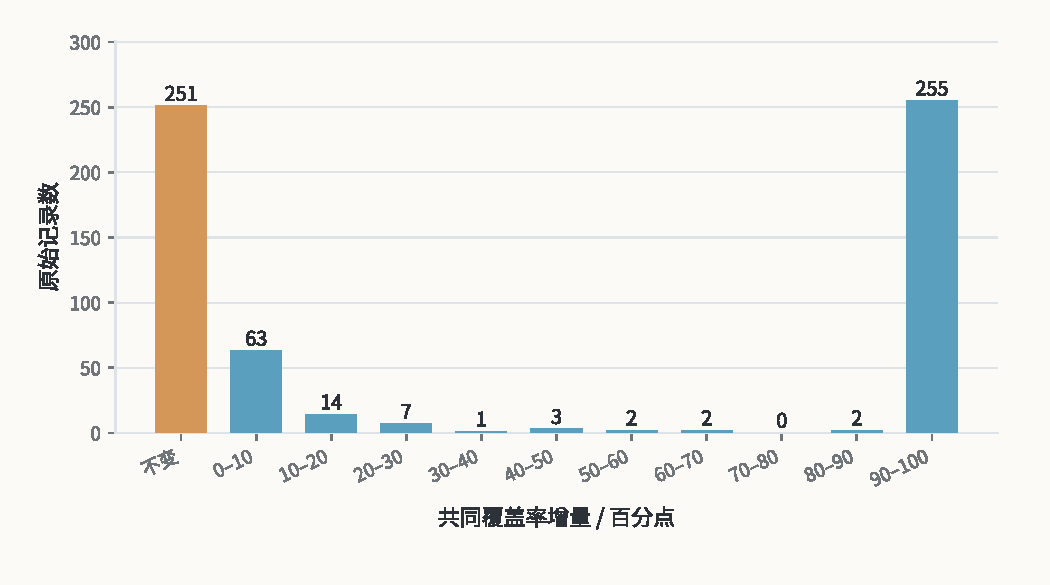
\includegraphics[width=.98\linewidth]{figures/confirmation_gain_histogram.pdf}
\caption{逐记录共同覆盖率的变化。零变化单独列出，其余按10个百分点分箱；统计单位为600条原始记录，100个百分点归入最后一组。覆盖增加不是噪声识别准确率增加。}\label{fig:confirm-hist}
\end{figure}

确认支持所选方案在这批记录和评价条件下采用，预设的参考回退没有触发。这不是再次选取赢家：如果结果不支持改善，就不能继续在同一批确认记录上调整参数。后续全量处理使用已经选定的固定设置，不逐记录调用模型、搜索或记忆。

\subsection{全量处理后，原始点去了哪里}
真实处理全部11,386条记录、1,173,410个点，包括早期开发与各评估分区。全量输出用于描述本数据集的处理结果，不作为另一批未见测试。参考与最终设置均形成25,963个片段，因为时间与距离切分阈值没有改变。

\begin{table}[htbp]\centering\small
\caption{全部轨迹的处理去向与结果}\label{tab:full}
\begin{tabularx}{\linewidth}{@{}Yrr@{}}\toprule
读数 & 参考设置 & 最终过滤调整\\\midrule
S短段过滤点 & 501,511 & 1,199\\
D方向删除点 & 36,056 & 39,732\\
P精简点 & 435,373 & 911,330\\
显式保留点 & 200,470 & 221,149\\\midrule
共同原始覆盖点 & 671,899 & 1,172,211\\
无输出记录 & 4,859 & 0\\
跨原始断点边 & 0 & 0\\\bottomrule
\end{tabularx}
\tabnote{前四项是互斥点去向，每列加总为1,173,410；覆盖与这些去向有重叠，不能再次相加。所有输入点均有终态，无处理失败、未处理记录或实际逐记录回退。}
\end{table}

最终方案相对参考增加500,312个共同覆盖点，只增加20,679个显式保留点。全量逐记录比较中，6,522条有严格改善，其余保持已有保护。图\ref{fig:flow}按同一原始点在两个方案中的状态连线，直接说明新增信息怎样进入后续处理。

\begin{figure}[H]\centering
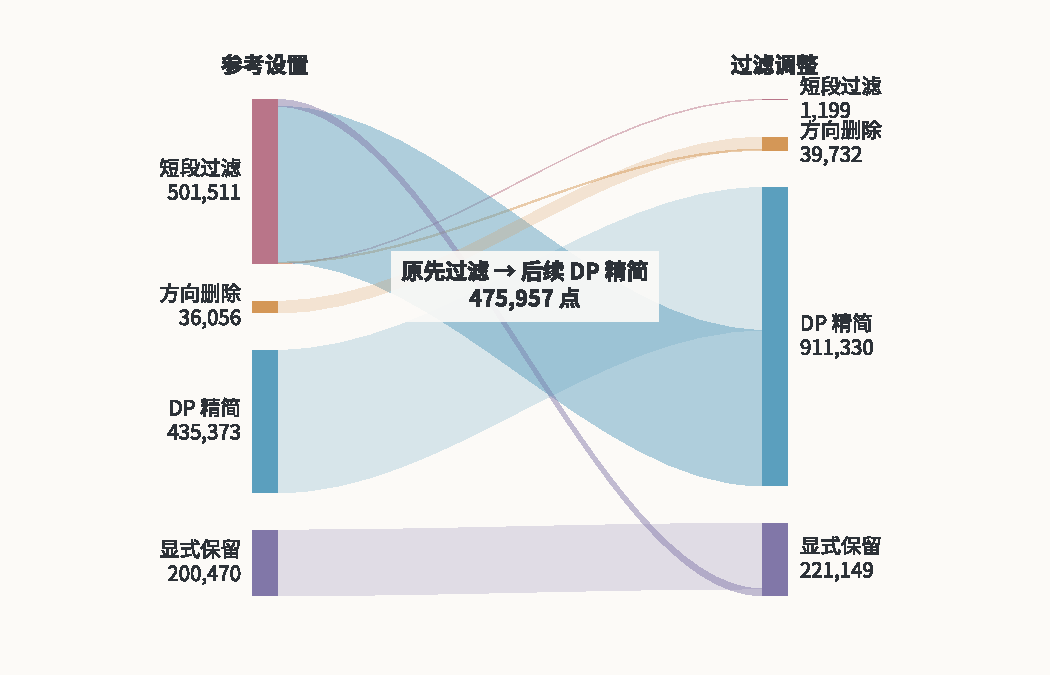
\includegraphics[width=\linewidth]{figures/point_fate_flow.pdf}
\caption{同一批原始点在两个方案中的去向对应。带宽按实际点数绘制；参考过滤掉的点中，475,957点在调整后进入DP精简，而非全部变成存储点。“覆盖”不是互斥终态，故未作为一条额外流加入。}\label{fig:flow}
\end{figure}

每个阶段的索引、坐标和时间均可与原始输入对应，汇总由实际点账本计算。全量的范围、终态和断点条件逐项检查；独立数值核对覆盖随机与边界记录，并保留最大误差案例。评价针对实际输出，而不是只让处理程序再次打印自身声称的统计。

\subsection{覆盖增加与存储量增加为何不同}
DP会用相邻保留点间的线段表示一些没有显式保存的原始点。因此，放宽过滤后，即使大量片段重新进入流程，也不需要原样存储全部点。表\ref{tab:added-cause}进一步将新增覆盖对应回参考过滤的具体原因。

\begin{table}[htbp]\centering\small
\caption{新增500,312个覆盖点原来被过滤的原因}\label{tab:added-cause}
\begin{tabularx}{\linewidth}{@{}Yr@{}}\toprule
参考过滤原因 & 新增覆盖点\\\midrule
仅累计长度不足 & 492,513\\
仅点数不足 & 5,434\\
点数与长度同时不足 & 2,365\\\midrule
合计 & 500,312\\\bottomrule
\end{tabularx}
\end{table}

主要收益来自减少长度下限引起的整段丢失。与此同时，过滤调整后的P输入有1,132,479点，参考只有635,843点，DP省点率分别约80.47\%与68.47\%。这两个百分比使用不同输入，不能写成DP算法提升了约12个百分点。

新的覆盖也不全是有意义的行驶轨迹。近静止观测、短片段乃至位置异常都可能重新被表达。当前结果支持减少参考过滤造成的信息损失；它没有直接评价停留语义、真实路径恢复或噪声识别准确率。

\subsection{较大偏差来自哪一步}
全量P即时最大误差约4.999964工作米，仍在5以内；原始覆盖点到最终折线的最大偏差却约368.707060工作米，两种方案的这一最大值相同。它们使用不同参考集合，因此并不矛盾。

新增覆盖中的最差点是记录352的原始索引105。所在窗口为104--107，共4点，累计长度约809.444工作米。参考因点数少于5过滤它，并非长度太短。过滤调整保留该段后，D删除105；P的输入与输出均为104、106、107，局部没有再删点。

\begin{figure}[H]\centering
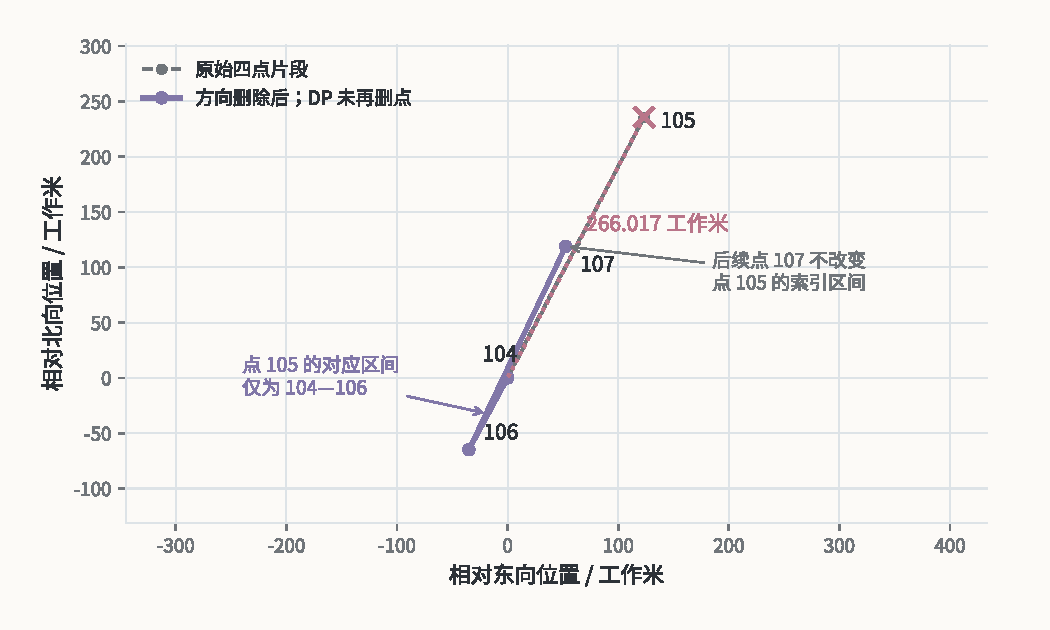
\includegraphics[width=.95\linewidth]{figures/boundary_record352.pdf}
\caption{记录352的局部边界案例。灰色虚线为原始四点片段，紫线为最终输出，玫瑰色虚线表示原始点105到对应最终线段的偏差。坐标只平移到104点，保持等比例；D删除的点不属于P即时输入。}\label{fig:boundary}
\end{figure}

点105按原始索引由104与106夹住，因此只在这条线段上计算偏差，不改取后续的106—107段。其距离为266.016754工作米。这个例子没有违反DP的输入误差定义，却说明覆盖恢复与原始形状完整保留仍然不同。现有资料也不能断言105是真实噪声或真实折返。保留这一案例，比只展示平滑后的成功轨迹更能限定最终结论。

全量坐标核对延续同一数学模型，没有把7条早期试运行的结果直接当成全域数值保证。独立转换核对用于检查实现，实际阈值敏感性另行检查；二者都不能反推源坐标基准。上述几何读数应当继续按工作米理解。
